\documentclass{winnower}

\begin{document}

\title{Speaker gender balance at Society for the Neurobiology of Language conferences 2009--2015}

\author{Jonathan E.\ Peelle}
\affil{Department of Otolaryngology, Washington University in Saint Louis, Saint Louis, Missouri 63110, USA}

\date{}

\maketitle

\begin{abstract}
I examined the gender balance of speakers at annual meetings of the Society for the Neurobiology of Language from 2009--2015, and in authors in the journal {\itshape Brain and Language} from the beginning of 2015. Of the conference speakers, 30\% (14/47) were women, with no year having more than 38\% speakers who were women. In contrast, approximately half of the authors (82/159) published in {\itshape Brain and Language} were women. These findings suggest intentional strategies are needed to achieve conference speaker gender balance.
\end{abstract}


\section{Introduction and Motivation}

Gender gaps in science are routinely documented in publishing, pay, hiring, and family (\cite{Shen2013}). As we plan future meetings of the Society for the Neurobiology of Language\footnote{\url{http://neurolang.org}} (SNL) the topic of speaker diversity has very sensibly been raised.  It is well established that most of us---including scientists of all genders---show unconscious bias (\cite{Raymond2013, Valian1999}), which contributes to gender disparities. Balance in the gender of conference speakers is one way to counter this unconscious bias.

As a first step in considering what we might want speaker gender balance to look like at future SNL meetings, it is useful to look at the data on speakers at prior meetings (\cite{Martin2014}). In that spirit, I have put together this summary of previous SNL speakers.

To provide some context for the gender distribution in the field of the neurobiology of language, I have looked at authors in {\itshape Brain and Language}, a speciality journal closely aligned with the interests of SNL. There are sensible arguments to be made for equal gender representation in conference speakers, regardless of the overall gender balance in a particular field. That is, even in a field that contains professionals of predominantly one gender, it is still beneficial to have equal gender representation, which can increase diversity of ideas and support junior academics who do not fit traditional stereotypes. Nevertheless, the ``overall gender distribution in a field'' is sometimes used to gauge the ease with which gender parity might be achieved.

I have uploaded all data and analysis to a public repository\footnote{\url{https://github.com/jpeelle/SNLspeakers}} so that others can view and contribute. When used, file names refer to files in this repository. Additional analyses and future extensions are very welcome!



\section{Data}

\subsection{SNL speaker data}


I obtained data on SNL speakers from PDFs of previous meeting programs.\footnote{downloaded from \url{http://www.neurolang.org/previous/} on October 19, 2015}

I created a spreadsheet listing speakers for each year, along with their gender, country, type of talk (keynote, debate, symposium), and so on, in {\ttfamily SNLspeakers\_data.tsv} (tab-delimited text file). The data cover 7 years, 2009--2015 inclusive.

I determined gender and country information based on my best guesses from the program and assumptions based on photos or first names. I judged board membership based on the current board published in the PDF program from each year.

Although the programs refer to ``panel'' discussions, I've used the term ``debate'', which is more common in practice when talking about past SNL meetings.

I did not include the 2014 symposium (``A neurobiology of naturalistic language use?'') as I believe this was contributed rather than invited, though the balance was similar to other talk categories (3/4 male speakers).


\subsection{{\itshape Brain and Language} Author Data}


I manually went through the first three volumes from 2015 of {\itshape Brain and Language} on the ScienceDirect website.\footnote{\url{http://www.sciencedirect.com/science/journal/0093934X/}} I entered basic article and author data in {\ttfamily author\_data.tsv}. I included all types of original research articles, but not errata. Again, I assigned gender based on likelihood given authors' first names or photos found on academic websites.


\subsection{Code}


All of the relevant R code is provided in the repository, meaning you should be able to paste in to an R console and recreate the numbers and plots. You can view the Rmarkdown source in the repository ({\ttfamily SNLspeakers.Rmd}) for a plain-text version. For plotting, I used the wonderful {\ttfamily divergingPips} package from Richard Morey.\footnote{\url{https://github.com/richarddmorey/divergingpips}}



\section{Results}

\subsection{SNL Speakers}

As shown in Figure 1, between 2009--2015 SNL has had 47 total speakers, of whom 14 (30\%) have been women. No year has had more than 38\% women speakers.

%%%%%%%%%%%%%%%%%%%%%%%%%%%%%%%%%%%%%%%%%%%%%%%%
\begin{figure*}
\begin{center}
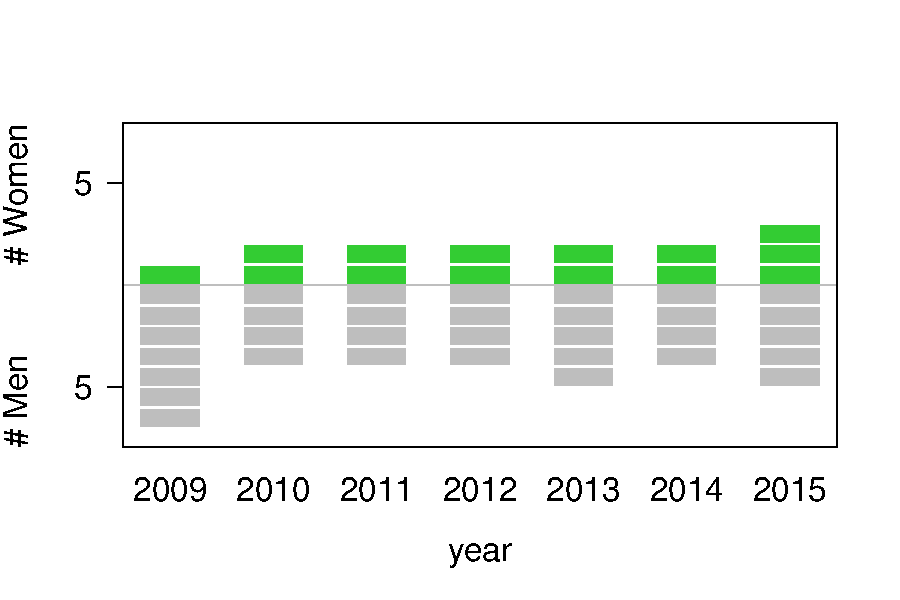
\includegraphics[scale=0.8]{SNLspeakerfigure.pdf}\vspace{0cm}
\caption
{Gender distribution of Society for the Neurobiology of Language conference speakers by year.}
\label{figSpeakers}
\end{center}
\end{figure*}
%%%%%%%%%%%%%%%%%%%%%%%%%%%%%%%%%%%%%%%%%%%%%%%%


The pattern is fairly similar across talk type, with the exception being equal gender representation in the 2015 invited symposium (debates: 6 women, 16 men; keynotes: 6 women, 16 men; symposium: 2 women, 2 men).



\subsection{{\itshape Brain and Language} Authors}

As seen in Figure 2, during the first three months of 2015 there were 159 authors published in {\itshape Brain and Language}, of whom 82 (52\%) were women. The breakdown was similar across author type (first author: 19 women, 13 men; middle author: 48 women, 48 men; last author: 15 women, 16 men).


%%%%%%%%%%%%%%%%%%%%%%%%%%%%%%%%%%%%%%%%%%%%%%%%
\begin{figure*}
\begin{center}
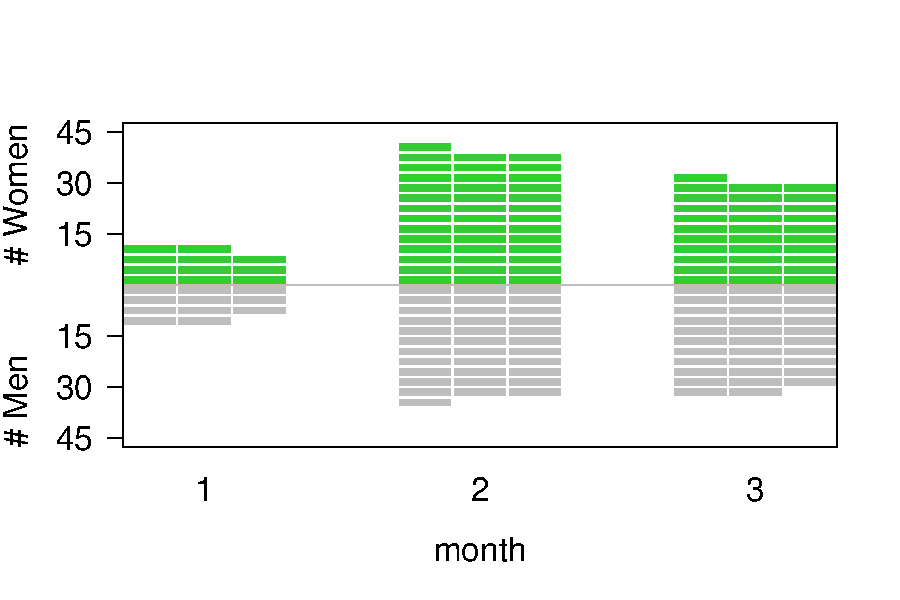
\includegraphics[scale=0.8]{BLauthorfigure.pdf}\vspace{0cm}
\caption
{Gender distribution of {\itshape Brain and Language} authors by month for January--March 2015.}
\label{figAuthors}
\end{center}
\end{figure*}
%%%%%%%%%%%%%%%%%%%%%%%%%%%%%%%%%%%%%%%%%%%%%%%%


\section{Comment}

For the first 7 years SNL has had an average 70/30 balance of male-to-female speakers. At first glance this 70/30 split does not appear to reflect the overall distribution of scientists in the field, which {\itshape Brain and Language} author data suggest is closer to 50\% women.

Although the primary aim of this document is to be descriptive rather than prescriptive, a few useful articles and blog posts on speaker diversity may help provide additional context and suggestions on achieving a more balanced set of conference speakers:

\begin{itemize}

\item The aforementioned Martin (2014) Ten simple rules to achieve conference speaker gender balance
\item ``Increasing diversity at your conference''\footnote{\url{http://www.ashedryden.com/blog/increasing-diversity-at-your-conference}} by Ashe Dryden
\item ``Suggestions for speaker diversity''\footnote{\url{http://phylogenomics.blogspot.com/2014/10/some-suggestions-for-having-diverse.html}} by Jonathan Eisen

\end{itemize}

One possible goal in conference organizing is to ensure approximately equal numbers of men and women speakers. Given that for the first 7 years 70\% of the SNL speakers have been men, if our goal were to have approximately equal numbers of men and women speakers overall, we should aim for 70\% women speakers for the next 7 years (through SNL in 2022).

(If that 70\% number sounds odd to you, it did to me also. But it did not seem nearly as odd to me as an attendee for most of the past 7 conferences when 70\% of the speakers were men. That mismatch is unconscious gender bias in a nutshell.\footnote{When asked about gender balance on the US Supreme court, Justice Ruth Bader Ginsberg responded: ``So now the perception is, yes, women are here to stay. And when I'm sometimes asked when will there be enough [women on the Supreme court]? And I say when there are nine, people are shocked. But there'd been nine men, and nobody's ever raised a question about that.''})

I have not looked at other types of speaker diversity, such as nationality, race/ethnicity, career stage, etc. These would be natural additional areas to include in future discussions on diversity and inclusiveness.


\bibliographystyle{abbrvnat}
\bibliography{Peelle_SNLspeakers}


\end{document}
